\chapter{Duet benchmarking}
\label{chap:duet}

Performance comparison of two different software versions is referred to as A/B benchmarking.
For example, compiler authors want to test if their optimization improved performance of some benchmark, or a web developers want to test if a recent commit caused regression in their internal benchmark.
In both cases the benchmark code is the same, and it runs with two slightly different workloads, versions A and B, that are similar in nature.

\Cref{fig:method_timeline} shows a comparison between three benchmarking methods analyzed in this thesis (1) sequential, (2) synchronous duet and (3) asynchronous duet.
The sequential method is the simplest where each version is run independently of the other.
Synchronous duet on the other hand runs A and B in parallel and it has to synchronize the starts of individual iterations.
Asynchronous duet runs in parallel as well but does not require synchronized iterations.

\begin{figure}
	\centering
	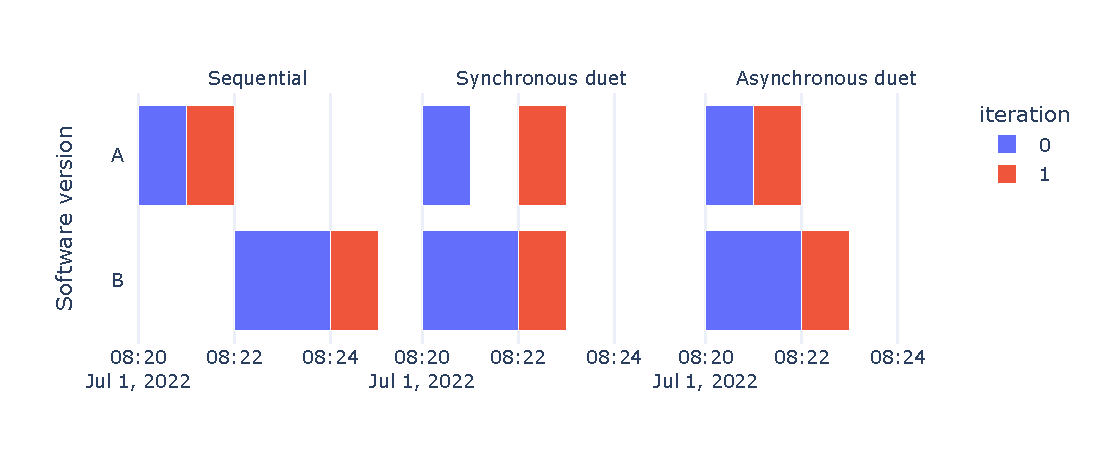
\includegraphics[width=.9\linewidth]{./figures/method_timeline.pdf}
	\caption{
	Comparison of different benchmarking methods sequential, synchronous duet, and asynchronous duet when comparing 2 software versions A and B.
	Benchmark runs 2 iterations with the same durations for all methods and versions.
	Note that version B introduced a regression where the first iteration takes twice as long.
	The \mbox{x-axes} is an example timeline of measurements.
	}
	\label{fig:method_timeline}
\end{figure}

% RQ1 Runtime reduction
The example in \cref{fig:method_timeline} has the durations of iterations equal for all methods, which illustrates one immediate benefit of running duet benchmarks --- overall runtime reduction.
In an ideal case, the duet method could save up to $50\%$ of execution run time and hence halve execution costs.
As this speedup is crucial for time and monetary reasons, we will investigate it thoroughly in this thesis.
A research question we would like to see answered is:

\begin{quote}
	\textbf{RQ1:} \emph{What are the runtime savings of the asynchronous duet method compared to the sequential method?}
\end{quote}

% Mutual interference
However, to achieve such speedup, workloads running in parallel must not interfere with each other.
To address mutual workload interference,~\citet{bulej2020duet} set up measurements in such a way that each benchmark was restricted to a single dedicated virtual core.
Even then, it may be the case that the two virtual cores map to the same hardware threads of the same physical core.
Such virtual cores would then compete for the single shared physical core.
Here~\citet{bulej2019initial} rely on workload symmetry.

Workload symmetry states that if a cloud were to exhibit systematic performance differences between the two virtual cores running duet workloads, it would likely exhibit similar unwarranted performance differences in other common concurrent workloads, such behavior would be likely considered a bug and remedied.
In other words, they rely on fair CPU scheduling~\footnote{Linux kernel uses "Completely Fair Scheduler" \url{https://en.wikipedia.org/wiki/Completely_Fair_Scheduler}} to work out mutual interference.
\citet{bulej2019initial} also note that this works only for similar workloads, which can be expected of neighboring commits or versions of the same software.

% External interference, Synchronized interference, Impact symmetry for seqn syncduet and async duet.

\section{Synchronous vs. Asynchronous duet}

% Impact symmetry on an asynchronous duet
\Cref{fig:method_timeline} also note that synchronized duet methods are not always running in parallel.
Once an iteration finishes it has to wait for its pair iteration to finish, until then, this pair iteration runs alone.
It might seem that an asynchronous duet solves this issue because iterations are not blocked on the barrier, so the only iteration running alone will be the last iteration of either A or B, whichever finishes last.

However, the asynchronous duet might be worse off in terms of equal impact symmetry on parallel workloads due to the ways benchmark harnesses and benchmarks themselves work.
\Cref{alg:harness} is a generic example of what an inner loop of a benchmark harness might look like.
Pre-iteration and post-iteration functions might do some environment checks like running garbage collection and recording or validating results.
Therefore, it is natural that these additional steps create gaps between measured code and that impacts asynchronous duet symmetry.

\begin{algorithm}
\begin{algorithmic}
	\Function{RunHarness}{$b$}
		\State \Call{Setup}{$b$}
		\For{$i \in 1 \dots I$}
		 	\State \Call{PreIteration}{}
			\State $start \gets$ \Call{clock.now}{}
			\State \Call{RunBenchmark}($b$)
			\State $end \gets$ \Call{clock.now}{}
			\State \Call{PostIteration}{$b$, $i$, $start$, $end$}
		\EndFor
		\State \Call{ValidateResults}{$b$}
		\State \Call{Teardown}{$b$}
	\EndFunction
\end{algorithmic}
\caption{
	Generic workings of the benchmark harness which executes a benchmark.
	Note that not all harnesses follow this structure --- some functions might be effectively empty.
	Specifically for synchronous duet~\citet{bulej2020duet} had to modify \emph{PreIteration} to wait on tabarrier.
}
\label{alg:harness}
\end{algorithm}

\Cref{fig:overlap_timeline} shows what implications can the absence of synchronization have on workload overlaps.
With enough iterations, harness specifics, and potentially different A/B performance workloads will inevitably diverge.

Even if workloads are partially overlapping, the start of a workload might do different things, for example, be CPU bound while the end of the workload might be I/O bound.
Fair CPU scheduling should, in theory, allocate the same amount of processor time for both workloads essentially synchronizing them.
However, in practice, due to the inherent variability of these systems workloads will diverge.

For example, \cref{fig:overlap_interference} demonstrates a case when this happens.
Even workloads with the same performance might get to a state of equilibrium where parts of workloads with different bound nature overlap each other.
This kind of symmetry can further hinder the impact symmetry argument for the synchronous duet method.
Therefore, our next research question examines the way duet pairs overlap:

% RQ2 Overlaps
\begin{quote}
	\textbf{RQ2:} \emph{How do workloads overlap in the asynchronous duet?}
\end{quote}

\begin{figure}
	\centering
	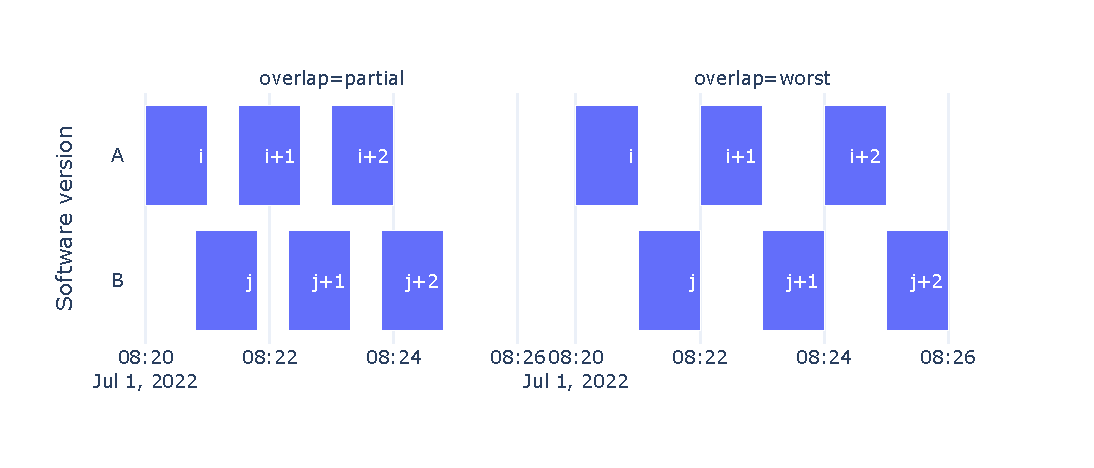
\includegraphics[width=.9\linewidth]{./figures/overlap_timeline.pdf}
	\caption{
		Tailored examples of how lack of synchronization and time in between workload execution might affect duet overlap.
		This is an example timeline of iterations of an \emph{asynchronous duet} measurement from an iteration $i$ and $j$ for versions $A$ and $B$ respectively.
		Focus on how versions $A$ and $B$ overlap --- just partially or even not at all.
	}
	\label{fig:overlap_timeline}
\end{figure}

\begin{figure}
	\centering
	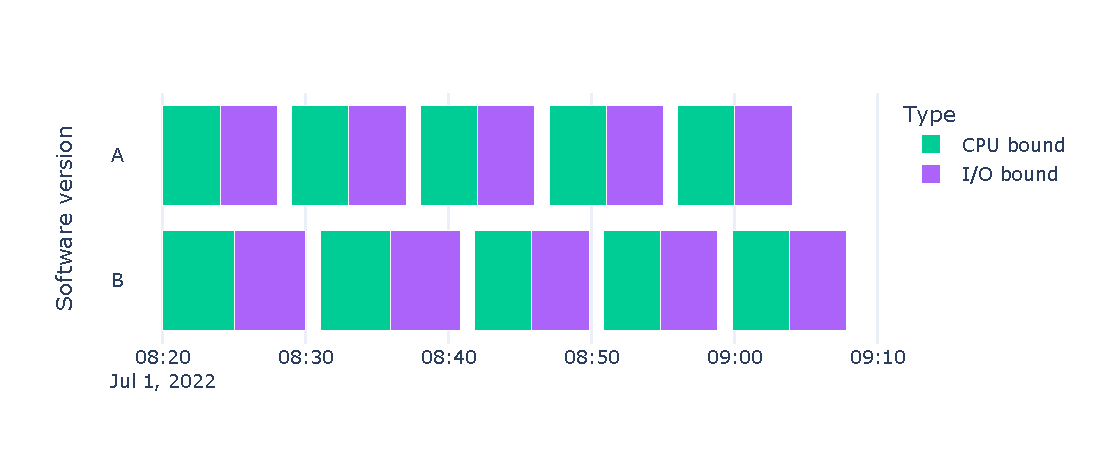
\includegraphics[width=.9\linewidth]{./figures/overlap_interference.pdf}
	\caption{
		Tailored examples of how different nature of a workload might compromise the duet's impact symmetry.
		Initially, $A$ and $B$ overlap on both CPU and I/O bound parts which slow down $B$ for the first 2 runs.
		Then, CPU and I/O bound parts of $A$ and $B$ workloads overlap less end $B$ turns out to be as fast as $A$.
		Notice that $A$ and $B$ enter a state of equilibrium where each is bound on different parts of the underlying hardware.
	}
	\label{fig:overlap_interference}
\end{figure}

For the asynchronous duet method to be useful runtime reduction and overlapping workloads are not enough.
The asynchronous duet method has to show accuracy in regression detection on par with the synchronized duet method:

% RQ3 Accuracy
\begin{quote}
	\textbf{RQ3:} \emph{What is the accuracy of regression detection of asynchronous duet compared to synchronous duet and sequential execution across different environments?}
\end{quote}

Additionally, using a similar approach to~\citet{laaber2019software} asynchronous and synchronous duet methods can be compared with sequential measurements in terms of \emph{minimal detectable slowdowns}~\cref{sec:mds}:

% RQ4 Minimal detectable slowdown
\begin{quote}
	\textbf{RQ4:} \emph{What are the minimal detectable slowdowns with the sequential, synchronous duet, and asynchronous duet measurements that we can detect with $95\%$ confidence?}
\end{quote}

% Why is it important - runtime reduction, volatile environment, no suite modification
\section{Goals}
\label{sec:goals}

To summarize, these are the areas of focus for this thesis:
\begin{description}
	\item[Accessibility]
		Asynchronous duet relaxes the synchronized iteration requirement on benchmark harnesses imposed by the synchronized duet method.
		Our goal is to create a generic benchmark super-harness for running benchmarks from various suites using sequential and duet methods and automate the result processing.
	\item[Runtime and Cost reduction]
		Duet methods have the potential to drastically reduce, up to $50\%$, the execution time of benchmarks (RQ1).
	\item[Accuracy]
		The synchronized duet method can reduce the variance of benchmark results measured in a volatile environment, such as a public cloud~\cite{bulej2020duet}.
		The question is if the asynchronous duet can do the same (RQ2, RQ3, RQ4).
\end{description}
